\documentclass[a4paper, 12pt, oneside]{article}
\usepackage[utf8]{inputenc}
\usepackage[margin=3cm, bindingoffset=1cm]{geometry}
\linespread{1.5}
\usepackage{float}
\usepackage{csquotes}
\usepackage{subfig}
\usepackage{graphicx}
\usepackage{indentfirst}
\usepackage{fancyhdr}
\usepackage{alphabeta}
\usepackage{algpseudocode}
\usepackage{algorithm}
\usepackage{hyperref}
\usepackage[T1]{fontenc}
\usepackage{listings}
\usepackage[htt]{hyphenat}
\usepackage{pgfplots}

\usepackage[
    backend=biber,
    sorting=none
]{biblatex}
\addbibresource{bibliography.bib}


\setlength{\parindent}{1cm}

\pagestyle{fancy}
\fancyhf{}
\fancyhead[C]{\textbf{\leftmark}}
\fancyfoot[C]{\thepage}
\renewcommand{\headrulewidth}{1pt}
\renewcommand{\footrulewidth}{1pt}
\renewcommand{\contentsname}{Indice}
\renewcommand{\figurename}{Fig.}

\usepackage[Conny]{fncychap}

  
\begin{document}
\begin{titlepage}
    \begin{center}
        \LARGE{\uppercase{Università degli Studi di Salerno}}\\
        \vspace{5mm}
    	\uppercase{\normalsize Dipartimento di Informatica }\\
    \end{center}
    \begin{figure}[H]
        \centering
        
\includegraphics[width=0.35\textwidth]{logo_unisa}
    \end{figure}
    
    \begin{center}
        \normalsize{Corso di \textbf{Penetration Testing and Ethical Hacking}}\\
    	\vspace{10mm}
    	\LARGE{\textbf{\textsc{NoobBox-1}:\\ Metodologie Utilizzate per il processo di Penetration Testing}}\\
    	\vspace{3mm}
        \large{\uppercase{Anno Accademico 2022/2023}}
    \end{center}

    \vspace{55mm}
    \noindent
    \begin{minipage}[t]{0.6\textwidth}
    	\textsc{Docente}:\\\textbf{Prof. Arcangelo Castiglione}
    	\vspace{10mm}\\
    \end{minipage}
    \hfill
    \begin{minipage}[t]{0.4\textwidth}\raggedleft
    	\textsc{Studente}: \\\textbf{Hermann Senatore}
    \end{minipage}
\end{titlepage}

\tableofcontents
\newpage

\section{Introduzione}
Questo documento si propone di raccogliere in maniera esaustiva tutte le operazioni che sono state compiute allo scopo di condurre l'analisi sull'asset vulnerabile \textsc{NoobBox-1}, disponibile sulla piattaforma VulnHub \cite{noobbox} e che fa uso di un sistema operativo \textbf{GNU\slash Linux}.

Tale documento costituisce il \textbf{Documento 2}, necessario per la consegna dell'attività progettuale del corso di \textbf{Penetration Testing and Ethical Hacking} ed assicura la \textbf{replicabilità} dell'intero processo sulla piattaforma utilizzata.

In particolare, questa sezione consiste una panoramica sull'asset che è stato analizzato e ci si sofferma sull'ambiente utilizzato per condurre l'analisi sull'asset stesso.

\subsection{Ambiente di lavoro}
La piattaforma sulla quale è stato svolto l'intero processo consiste in un \textbf{MacBook Air} (late 2020) che utilizza il processore Apple Silicon M1 e che fa uso dell'architettura \textbf{arm64}. Anche se questa informazione al momento può apparire come di poco conto, diventerà rilevante durante la fase di Vulnerability Mapping ed in particolare al momento dell'installazione dei tools necessari. Ulteriori informazioni sul topic saranno fornite più avanti in questo documento.

Per condurre concretamente l'indagine sono state sfruttate due macchine virtuali utilizzando l'\textit{hypervisor} \textbf{UTM}, che utilizza \textbf{QEMU} come suo backend.

In particolare:

\begin{itemize}
    \item La prima macchina virtuale consiste nella versione \textbf{aarch64} del sistema operativo \textbf{Kali Linux};
    \item La seconda macchina virtuale consiste invece nell'asset vulnerabile menzionato poc'anzi.
\end{itemize}.

Di seguito sono presenti alcuni dettagli su entrambe le macchine.

\subsubsection{Macchina virtuale 1: dettagli}
La prima macchina virtuale è stata creata in maniera standard utilizzando l'immagine ISO reperibile presso il sito web della distribuzione \cite{kali}. La versione utilizzata risulta essere la \textbf{2023.1}, rilasciata il 13 marzo 2023. 

In fase di installazione è stato necessario adottare alcuni accorgimenti suggeriti nella relativa documentazione dell'\textit{hypervisor} utilizzato \cite{kali-utm}. Le informazioni presenti in questa pagina sono state create per le versioni \textbf{2022.x} ma sono valide anche per la versione utilizzata durante questo processo.

La macchina virtuale in questione utilizza il kernel Linux 6.1 e di seguito è presente l'output del comando \verb|uname -a|.

\begin{figure}[h]
    \centering
    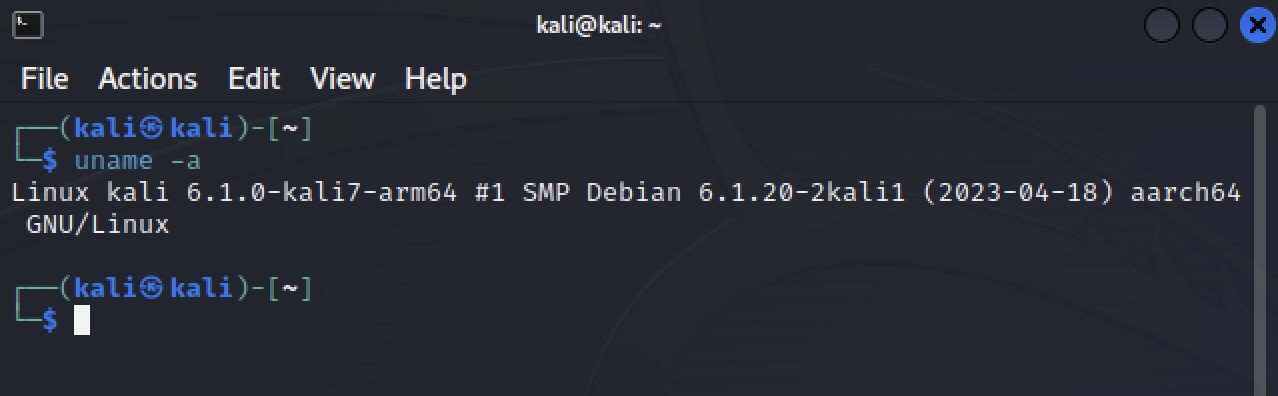
\includegraphics[scale=0.5]{img/uname.png}
    \caption{La versione del kernel utilizzata da Kali}
\end{figure}

\subsubsection{Macchina virtuale 2: dettagli}
Come menzionato in precedenza, la seconda macchina consiste proprio nell'asset su cui deve essere condotta l'analisi. Originariamente pensato per essere una sfida CTF, sulla piattaforma VulnHub viene rivelata la presenza di due \textit{flags} a cui accedere: una per l'utente non privilegiato ed una per \texttt{root}. 

Naturalmente, allo scopo di questo progetto non ci si è limitati alla cattura delle flag ma è stato seguito un approccio più sistematico che prevede l'utilizzo di tools e di metodologie standard tipiche di un processo di Penetration Testing.

Sulla piattaforma VulnHub viene offerto il download di NoobBox-1 in formato \texttt{.ova}, compatibile con il software \textbf{Oracle VirtualBox}. Tuttavia, al momento della stesura di questo documento, non esiste una versione nativa di tale software per la piattaforma Apple Silicon in uso e l'hypervisor d'elezione non supporta l'importazione di file \texttt{.ova}. 

Di conseguenza, si è reso necessario un ulteriore step di conversione per rendere tale macchina virtuale utilizzabile con \textbf{UTM} \cite{qcow}. Tale step consiste nella conversione dell'immagine disco in formato \texttt{.vmdk} presente all'interno del file \texttt{.ova} nel formato \texttt{.qcow2}, utilizzato dal software \textbf{QEMU} e quindi da \textbf{UTM}.

Gli step seguiti per la conversione dell'immagine disco sono riportati qui di seguito:

\begin{enumerate}
    \item Installazione di QEMU in maniera \textit{system-wide} usando il package manager \textbf{Homebrew}: \verb|brew install qemu|;
    \item Conversione dell'immagine disco usando il tool \textbf{qemu-img}.
    \begin{center}
        \verb|qemu-img convert -f vmdk -O qcow2 NoobBox-disk001.vmdk NoobBox-disk.qcow2|.
    \end{center}
    Lo switch \texttt{-f} permette di esplicitare il formato \textbf{sorgente}, mentre lo switch \texttt{-O} quello di \textbf{output}.
\end{enumerate}

Successivamente, è stato possibile creare una nuova macchina virtuale \textbf{Linux} e, conseguentemente, importare il file appena creato come disco virtuale. 

\newpage
\printbibliography[title={Riferimenti bibliografici e risorse consultate}]
\end{document}